\documentclass{beamer}
\usepackage{beamerthemesplit}
% \usepackage{pstricks}
\usepackage{graphicx}
\usepackage{mdwlist}
\usepackage{lineno, hyperref}

\usepackage{amssymb,latexsym,amsmath,amsthm,bbm}
\usepackage{hyperref}
\usepackage{tikz}
\usepackage[english]{babel}
\usepackage[latin1]{inputenc}
\usepackage{multirow}
\usepackage{verbatim}
\usepackage{alltt}
\usepackage{mycommands}

\usepackage{cmbright}
\renewcommand*\familydefault{\sfdefault}
\usepackage[T1]{fontenc}


\definecolor{wp-red}{RGB}{204,0,0}
\definecolor{wp-gray}{RGB}{51,51,51}
\definecolor{reynolds-red}{RGB}{153,0,0}
\definecolor{pyroman-flame}{RGB}{209,81,34}
\definecolor{hunt-yellow}{RGB}{253,215,38}
\definecolor{genomic-green}{RGB}{125,140,31}
\definecolor{innovation-blue}{RGB}{66,126,147}
\definecolor{bio-indigo}{RGB}{65,86,161}

\setbeamercolor{structure}{fg=wp-red}
\setbeamercolor{title}{bg=white, fg=wp-red}  % changes color on title page
\setbeamerfont{title}{series=\bfseries, size=\huge}
\setbeamerfont{author}{series=\bfseries, size=\large}
\setbeamerfont{institute}{series=\mdseries, size=\large}

\setbeamercolor{frametitle}{bg=wp-red, fg=white}  % changes color at top of frame
\setbeamerfont{frametitle}{series=\bfseries}
\setbeamercolor{title in head/foot}{fg=white, bg=wp-red}  % changes color for title in footer
\setbeamerfont{title in head/foot}{series=\bfseries}
\setbeamercolor{author in head/foot}{fg=white,bg=wp-gray}  % changes color for author in footer
\setbeamerfont{author in head/foot}{series=\bfseries}


\title[Spatiotemporal Modeling of Extreme Events] % (optional, use only with long paper titles)
{
  Spatiotemporal Modeling of Extreme Events
}
\author[S. Morris, B. Reich, and D. Cooley]{Samuel Morris (NC State), Brian Reich (NC State), and Dan Cooley (Colorado State)}
\institute[NCSU, CSU]{}
\date{JSM 2014, Boston}

\begin{document}

\begin{frame}\frametitle{\ }
\begin{center}
	\maketitle
\end{center}
\end{frame}

\begin{frame}{Motivation}
  \begin{itemize} \setlength{\itemsep}{1em}
    \item Average behavior is important to understand, but it does not paint the whole picture.
    \begin{itemize}
      \item e.g. When constructing river levees, engineers need to be able to estimate a 100-year or 1000-year flood levels.
    \end{itemize}
    \item Spatial extreme borrows strength across space to estimate return levels and make predictions at unknown locations..
    \item In geostatistical analysis, kriging uses spatial correlation for prediction.
    \item Want to explore similar methods for extremes.
  \end{itemize}
\end{frame}

% \begin{frame}{Introduction to extremes}
%   \begin{itemize} \setlength{\itemsep}{0.5em}
%     \item Max-stable processes (Cooley et al., 2012):
%     \begin{itemize}
%       \item Consider a spatial process $x_t(\bs)$, $t = 1, \ldots, T$.
%       \item Let $M_T(\bs) = \left\{ \bigvee_{t=1}^T x_t(\bs_1), \ldots, \bigvee_{t=1}^T x_t(\bs_n) \right\}$
%       \item If there exists normalizing sequences $a_T(\bs)$ and $b_T(\bs)$ such
%       that for all sites, $\bs_i, i = 1, \ldots, d$,
%       \begin{align*}
%         a_T^{-1}(\bs) \left\{ M_T(\bs) - b_T(\bs) \right\} \converged Y(\bs)
%       \end{align*}
%       which has a non-degenerate distribution, then $Y(\bs)$ is a max-stable process.
%     \end{itemize}
%   \end{itemize}
% \end{frame}

\begin{frame}{Standard analysis - Block maxima}
  \begin{itemize} \setlength{\itemsep}{0.5em}
      \item Uses yearly maxima
      \item Discards many observations
      \item Models are fit using the generalized extreme value distribution
    \item For a spatial analysis, max-stable processes give an appropriate limiting distribution
  \end{itemize}
\end{frame}

\begin{frame}{Standard analysis - Peaks over threshold}
  \begin{itemize}
      \item Incorporates more data than block maxima
      \item Select a threshold, $T$, and fit data above the threshold using the generalized Pareto distribution
      \item Temporal dependence may be an issue between observations (e.g. flood levels don't dissipate overnight)
    \item Generalized Pareto distribution (GPD) is used for the exceedances.
  \end{itemize}
\end{frame}

% \begin{frame}{Multivariate representations}
%   \begin{itemize}
%     \item Multivariate distributions:
%     \begin{itemize}
%       \item Assume common standardized max-stable marginal, like unit-Fr\'{e}chet
%       \begin{align*}
%         \Pr(Z < z) = exp(-z^{-1})
%       \end{align*}
%       \item The multivariate representation for the GEV is
%       \begin{align*}
%         \Pr(\bZ \le \bz)  &= G^*(\bz) = \exp(-V(\bz))\\
%                 V(\bs)    &= d \int_{\Delta_d} \bigvee_{i = 1}^d \frac{w_i}{z_i} H(\ddd w)
%       \end{align*}
%       where
%       \begin{itemize}
%         \item $\Delta_d = \{ \bw \in \calR^d_+ \mid w_1 + \cdots + w_d = 1\}$
%         \item $H$ is a probability measure on $\Delta_d$
%         \item $\int_{\Delta_d}w_i H(\ddd w) = 1 / d$ for $i = 1, \ldots, d$.
%       \end{itemize}
%     \end{itemize}
%   \end{itemize}
% \end{frame}

\begin{frame}{Multivariate analysis}
  \begin{itemize} \setlength{\itemsep}{0.5em}
    \item Multivariate max-stable and GPD models have nice features, but they are
    \begin{itemize}
      \item computationally challenging to work with
      \item joint distribution only available in low dimension
    \end{itemize}
    \item Pairwise likelihood approach (Huser and Davison, 2014)
  \end{itemize}
\end{frame}

\begin{frame}{Model objectives}
  \begin{itemize} \setlength{\itemsep}{0.5em}
    \item Our objective is to build a model that
    \begin{itemize}
      \item has marginal distribution with a flexible tail
      \item has asymptotic spatial dependence
      \item has computation on the order of Gaussian models for large space-time datasets
    \end{itemize}
  \end{itemize}
\end{frame}

\begin{frame}{Thresholding data}
  \begin{itemize} \setlength{\itemsep}{0.5em}
    \item We threshold the observed data at a high threshold $T$.
    \item Thresholded data:
    \begin{align*}
      Y_t^*(\bs) = \left\{ \begin{array}{ll}
          Y_t(\bs) \quad & Y_t(\bs) > T\\
          T \quad & Y_t(\bs) \le T
      \end{array}\right.
    \end{align*}
    \item Allows tails of the distribution to speak for themselves.
  \end{itemize}
\end{frame}

\begin{frame}{$\chi$ coefficient}
  \begin{itemize} \setlength{\itemsep}{0.5em}
   \item The $\chi$ coefficient is a measure of extremal dependence
   \item Specifically, we focus on $\chi(\bh)$ for the upper tail given by
    \begin{align*}
      \chi(\bh) = \lim_{c \rightarrow \infty}\Pr(Y(\bs) > c \mid Y(\bs + \bh) > c)
    \end{align*}
    \item If $ \chi(\bh) = 0$, then observations are asymptotically independent at distance $\bh$.
    \item We expect $\lim_{\bh \rightarrow \infty}\chi(h)=0$.
  \end{itemize}
\end{frame}

\begin{frame}{Gaussian spatial model}
  \begin{itemize} \setlength{\itemsep}{0.5em}
    \item In geostatistics $Y(\bs)$ are often modeled using a Gaussian process with mean function $\mu(\bs)$ and covariance function
$\rho(\bh)$.
    \item Model properties:
    \begin{itemize}
      \item Nice computing properties (closed-form likelihood)
    \item For a Gaussian spatial model $\lim_{c \rightarrow \infty} \chi(c) = 0$ regardless of the strength of the correlation in the bulk of the distribution.
    \item Tail is not flexible (Gaussian is light tailed)
    \end{itemize}
    \end{itemize}
\end{frame}

\begin{frame}{Spatial skew-$t$ distribution}
  \begin{itemize} \setlength{\itemsep}{0.5em}
    \item Assume observed data $Y_t(\bs)$ come from a skew-$t$ (Zhang and El-Shaarawi, 2012)
    \begin{align*}
      Y_t(\bs) = X_t(\bs)\beta + \alpha z_t + v_t(\bs)
    \end{align*}
    where
    \begin{itemize} \setlength{\itemsep}{0.25em}
      \item $\alpha \in \calR$ controls the skewness
      \item $z_t \iid N_{(0, \infty)}(0, \sigma^2_t)$ is a random effect
      \item $v_t(\bs)$ is a Gaussian process with variance $\sigma^2_t$ and \Matern correlation
      \item $\sigma_t^2 \iid \text{IG}(a, b)$
    \end{itemize}
  \end{itemize}
\end{frame}

\begin{frame}{Spatial skew-$t$ distribution}
  \begin{itemize} \setlength{\itemsep}{0.5em}
   \item \alert{Conditioned} on $z_t$ and $\sigma^2_t$, $Y_t(\bs)$ is a Gaussian spatial model
    \item Can use standard geostatistical methods to fit this model.
    \item Predictions can be made through Kriging.
    \item \alert{Marginalizing} over $z_t$ and $\sigma^2_t$ (via MCMC),
    \begin{align*}
      Y_t(\bs) \sim \text{skew-t}(\mu, \Sigma^*, \alpha, \text{df}=2a)
    \end{align*}
    where
    \begin{itemize}
    	\item $\mu$ is the location
	\item $a$, $b$ are the IG parameters for $\sigma^2_t$
	\item $\Sigma^* = \frac{ b }{ a } \Sigma$ is a scale matrix, and $\Sigma$ is a \Matern covariance matrix
	\item $\alpha \in \calR$ controls the skewness
    \end{itemize}
  \end{itemize}
\end{frame}

\begin{frame}{Spatial skew-$t$ distribution}
  \begin{itemize} \setlength{\itemsep}{0.5em}
      \item Model properties
    \begin{itemize}
    	\item Has flexible tail controlled by skewness $\alpha$ and degrees of freedom $2a$
    	\item For a skew-$t$ distribution $\lim_{c \rightarrow \infty} \chi(c) > 0$ Padoan, 2011)
    	\item Computation that is on the order of Gaussian computation
    \end{itemize}
    \item For this distribution, $\chi(\bh)$ shows asymptotic dependence that does not approach 0 as $\bh \rightarrow \infty$ 
   \item This occurs because all observations (near and far) share the same $z_t$ and $\sigma_t^2$.
    \item We deal with this through a daily random partition (similar to Huser and Davison).
  \end{itemize}
\end{frame}

\begin{frame}{Daily random partition}
  \begin{itemize} \setlength{\itemsep}{0.5em}
    \item Daily random partition allows $z_t$ and $\sigma^2_t$ to vary by site.
    \begin{align*}
      Y_t(\bs) = X_t(\bs) \beta + \alpha z_t(\bs) + \sigma(\bs) v_t(\bs)
    \end{align*}
    \item Consider a set of daily knots $w_{tk} \sim$ Uniform that define a random daily partition
    $P_{t1}, \ldots, P_{tK}$ such that
    \begin{align*}
      P_{tk} = \{s : k = \argmin_\ell|| \bs - w_{t\ell}|| \}
    \end{align*}
    \item For $\bs \in P_{tk}$
    \begin{align*}
      z_t(\bs) &= z_{tk}\\
      \sigma^2_t(\bs) &= \sigma^2_{tk}
    \end{align*}
    \item Within each partition $Y_t(\bs)$ has the same MV skew-t distribution as before.
  \end{itemize}
\end{frame}

\begin{frame}{Example daily partition}
	Two sample partitions (number is at partition center)
    \centering
    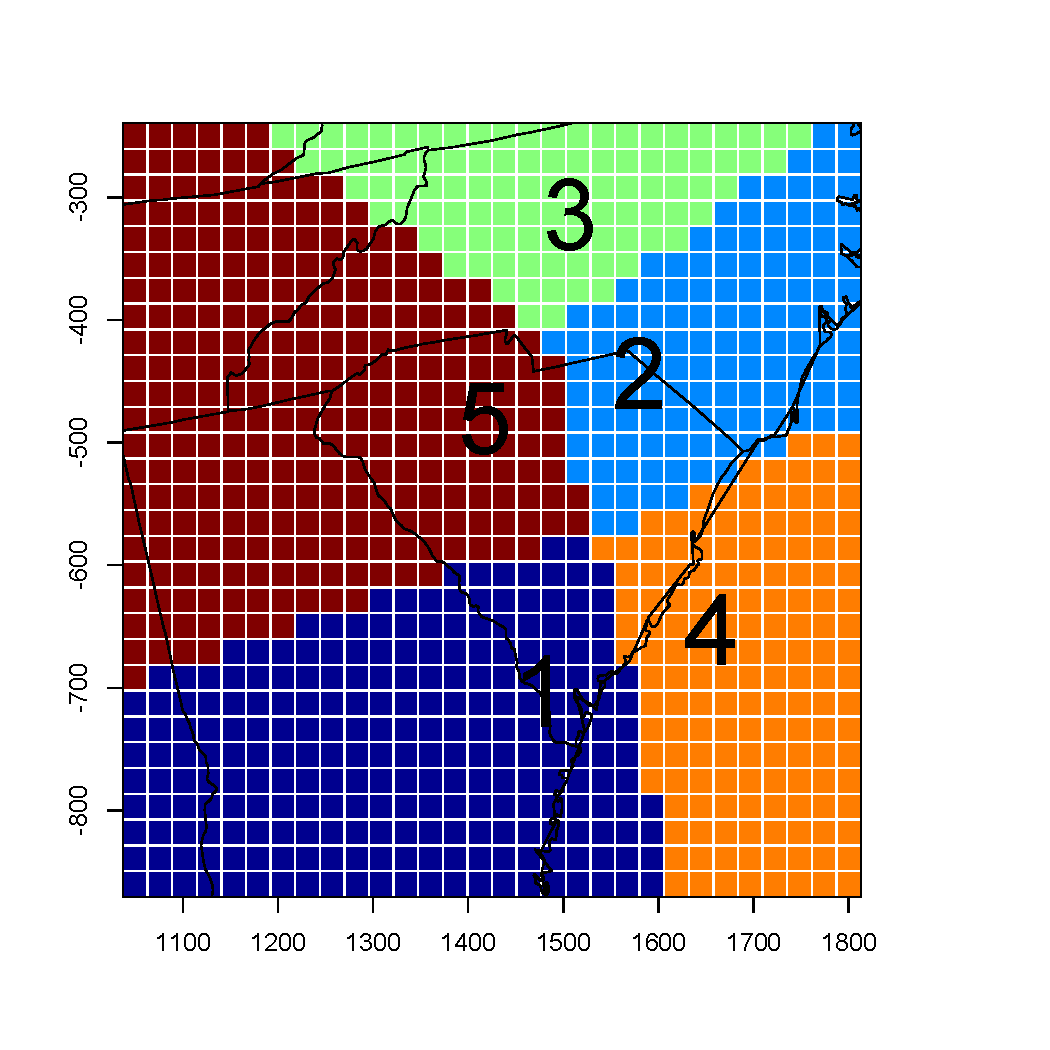
\includegraphics[width=0.54\linewidth]{./plots/example-partition-1.pdf}
    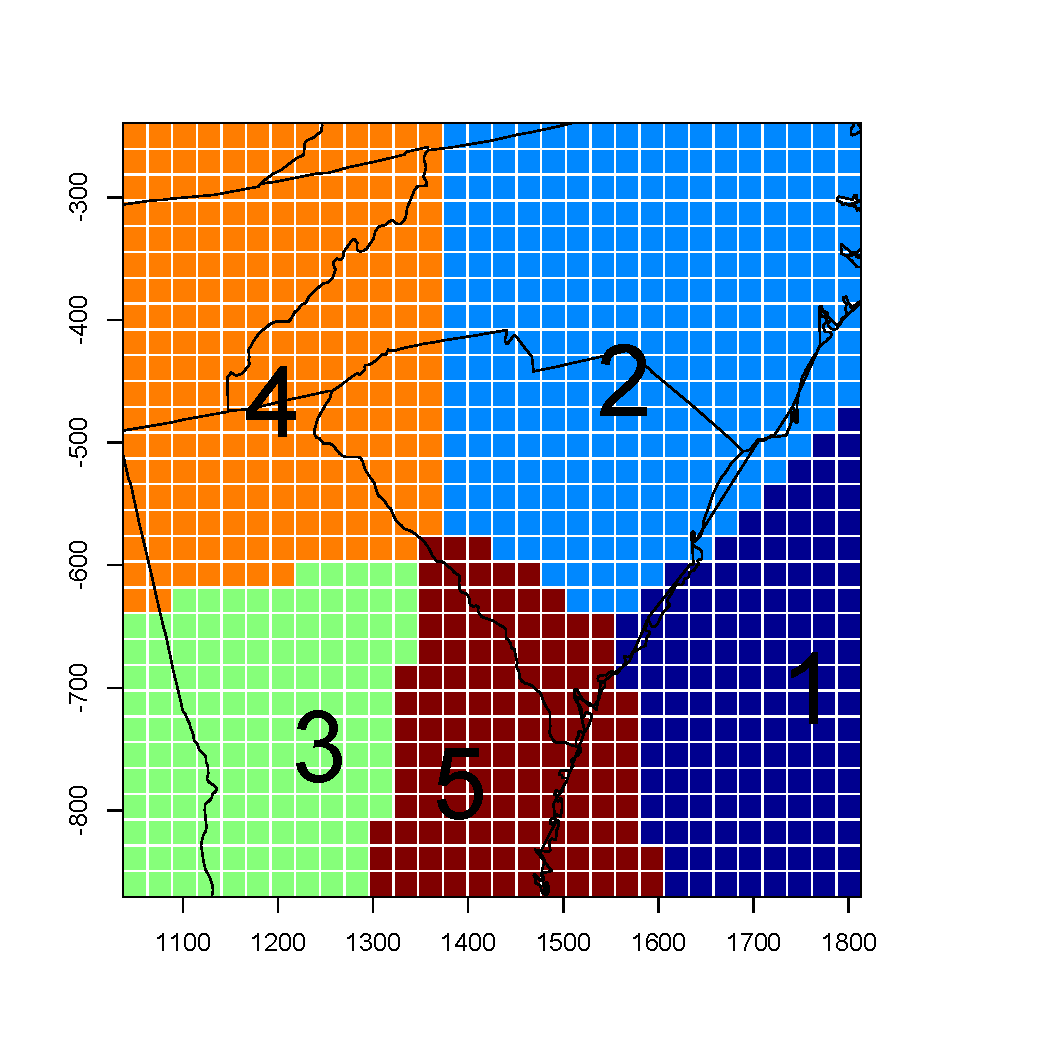
\includegraphics[width=0.54\linewidth]{./plots/example-partition-2.pdf}
\end{frame}


\begin{frame}{Simulated $\chi$ plots}
  \centering
  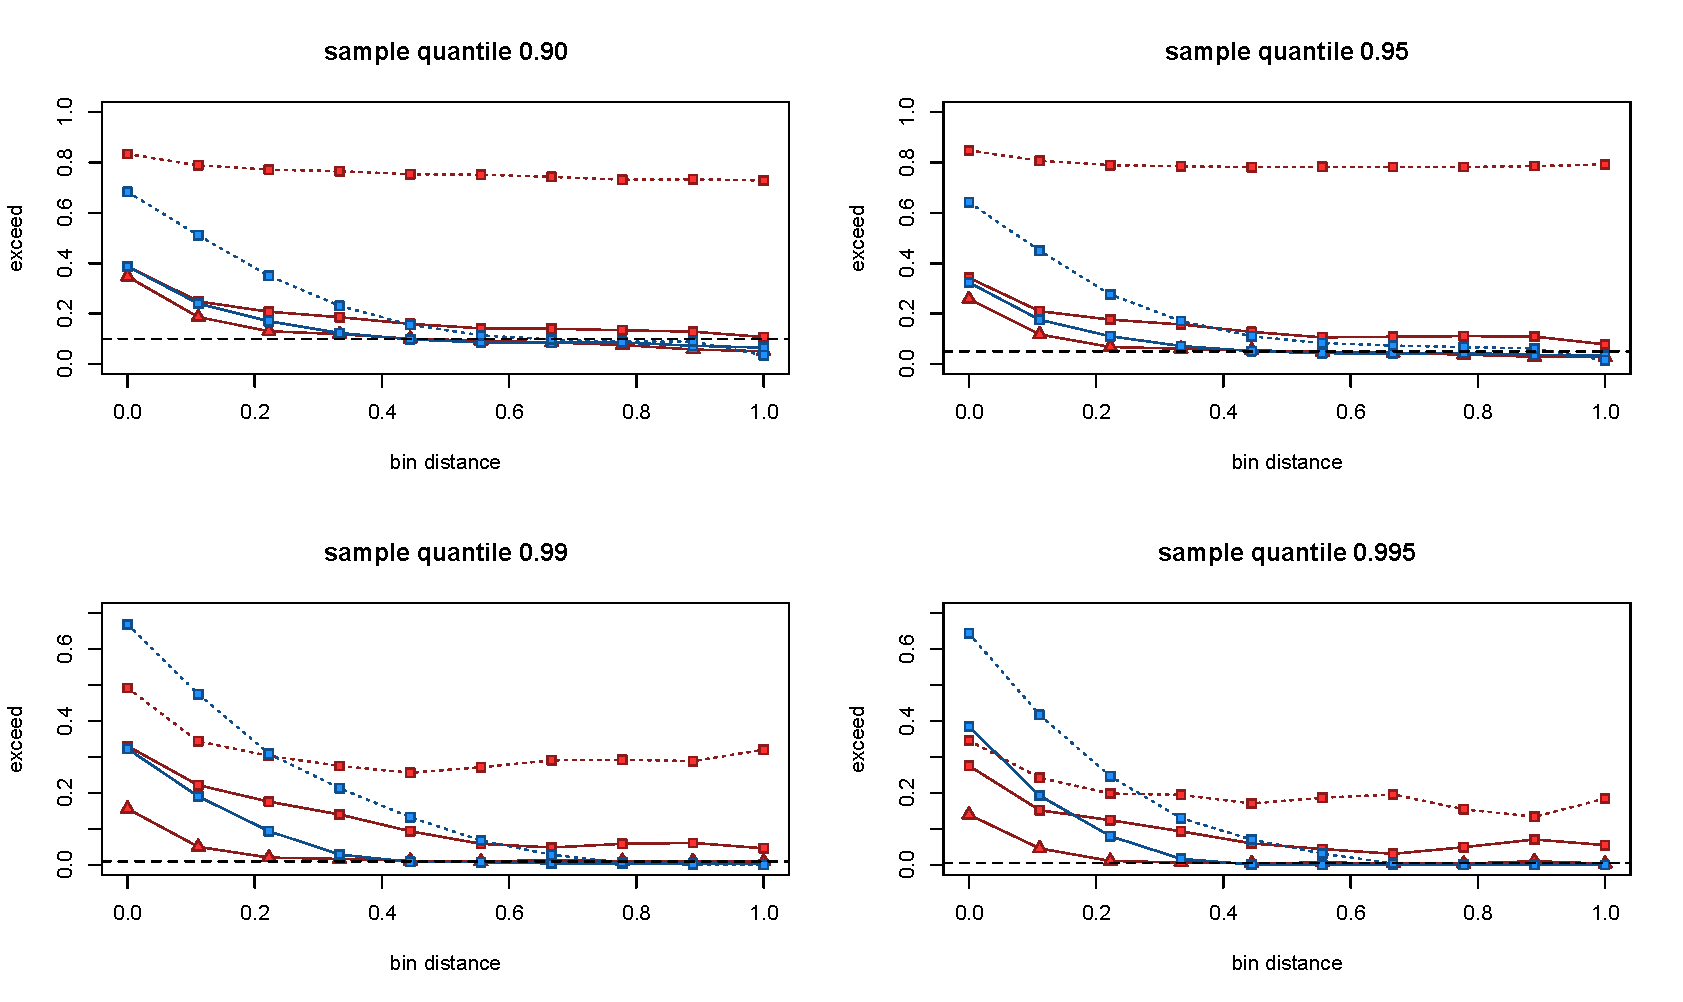
\includegraphics[width=1\linewidth]{./plots/chi-plots.pdf}\\[-0.25in]
  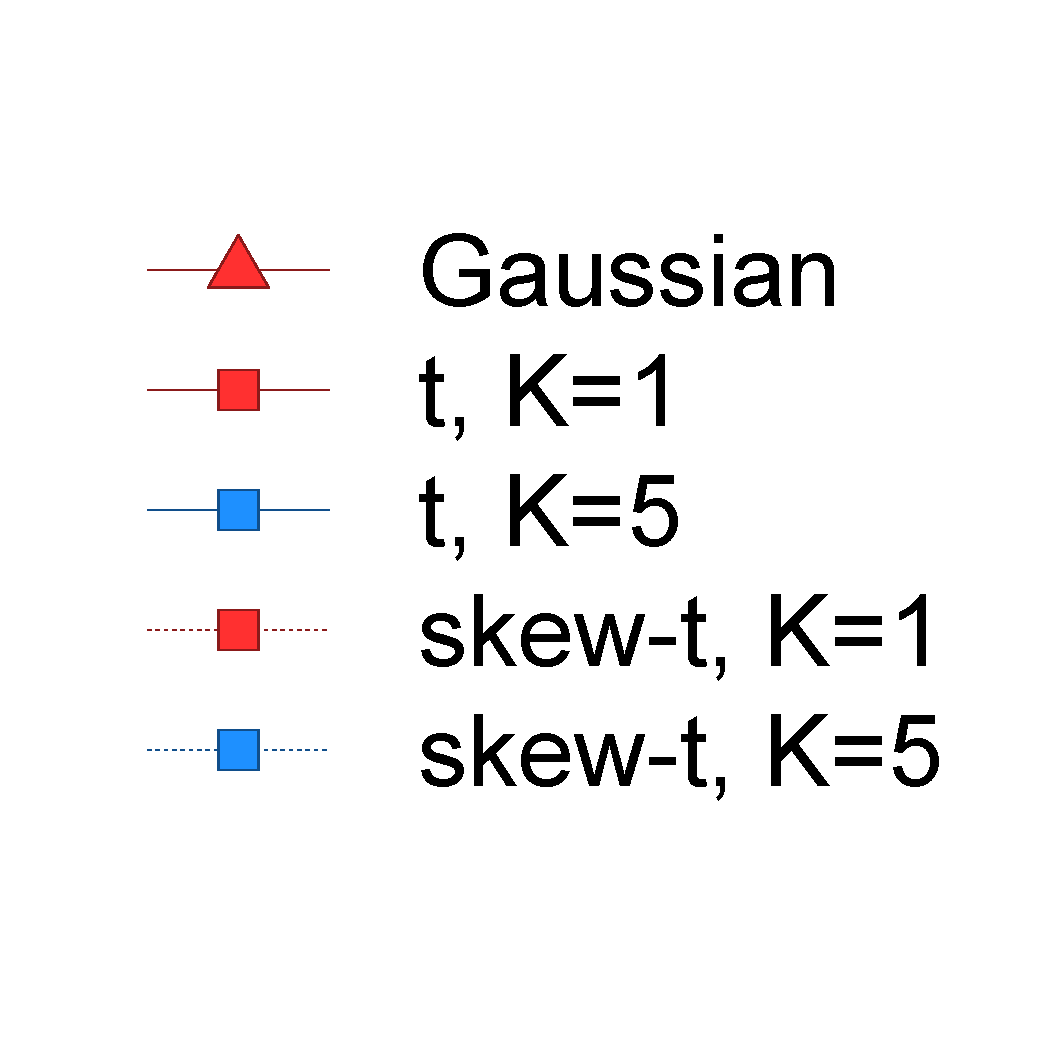
\includegraphics[width=0.2\linewidth]{./plots/chi-legend.pdf}
\end{frame}


\begin{frame}{Sample simulated datasets}
  \centering
  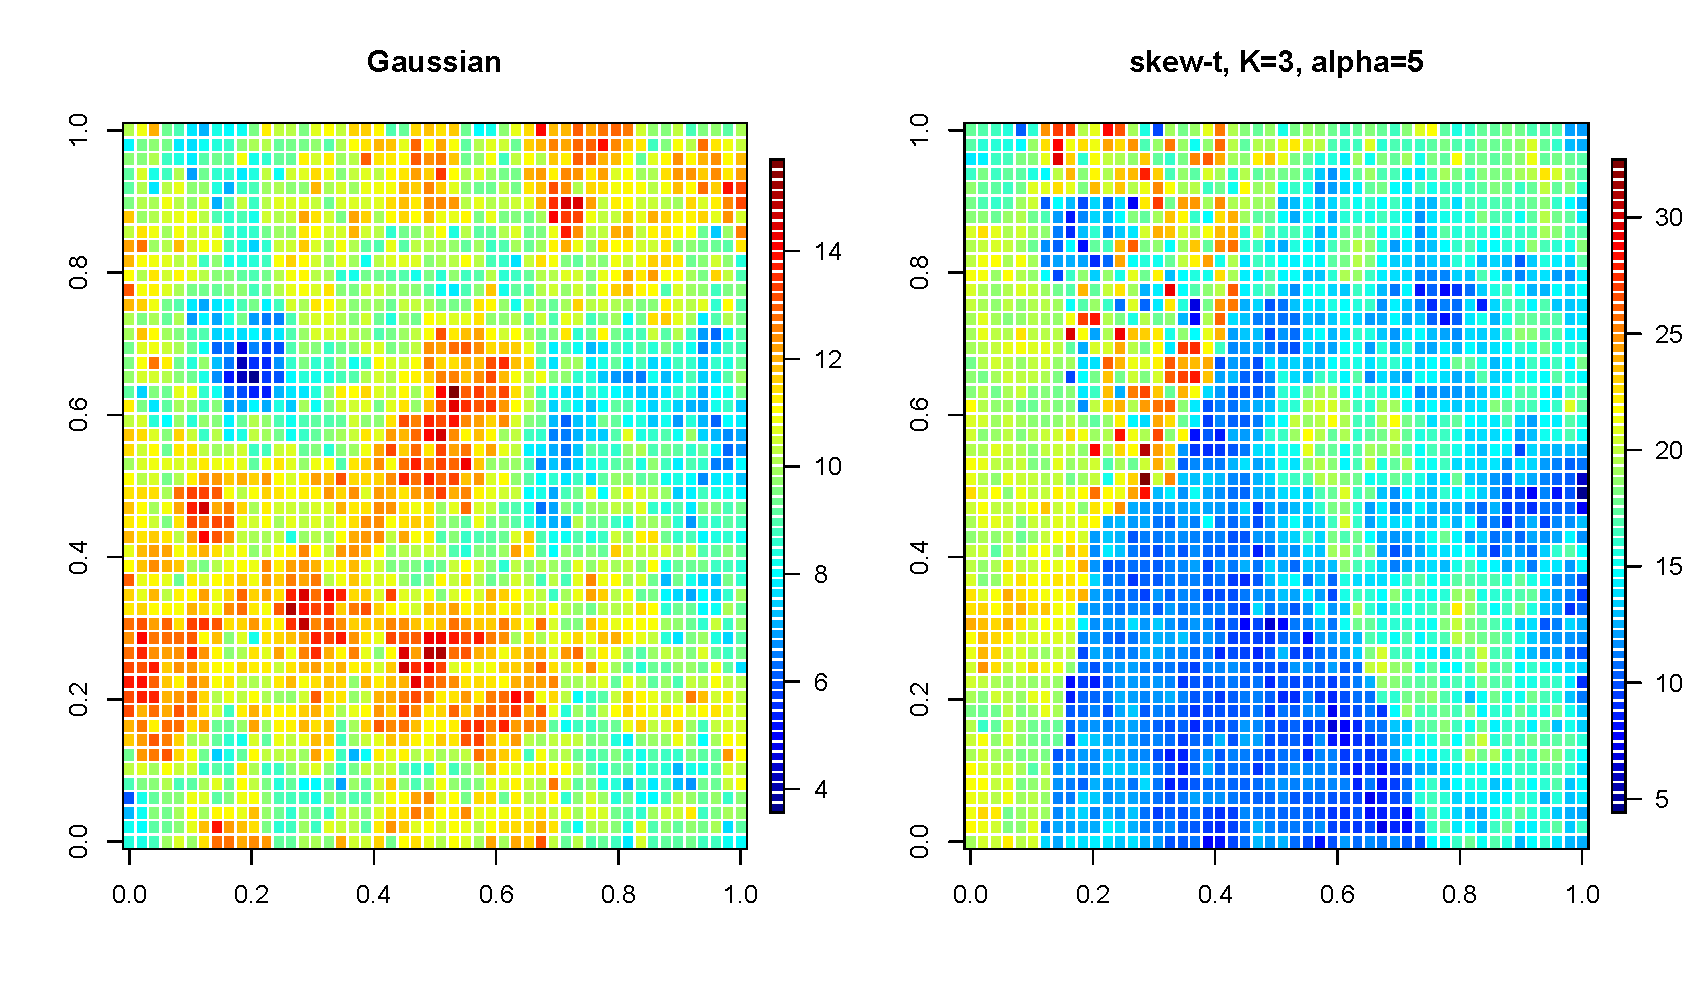
\includegraphics[width=1\linewidth]{./plots/gauss-vs-skew-t3.pdf}
\end{frame}

\begin{frame}{Spatiotemporal Model}
  \begin{itemize} \setlength{\itemsep}{0.5em}
    \item We can account for time in one of two ways
    \begin{itemize}
    	\item The mean: e.g. AR(1)
	\item Three dimensional covariance model (e.g. Huser and Davison, 2014) 
    \end{itemize}
  \end{itemize}
\end{frame}

\begin{frame}{MCMC details}
  \begin{itemize} \setlength{\itemsep}{0.5em}
    \item Three main steps:
    \begin{enumerate}[1.]
      \item Impute missing observations and censored data below $T$
      \item Update parameters with standard random walk Metropolis Hastings or Gibbs sampling
      \item Make spatial predictions
    \end{enumerate}
    \item Priors are selected to be conjugate when possible.
  \end{itemize}
\end{frame}

\begin{frame}{Data analysis}
	\centering
	Ozone monitoring station locations
    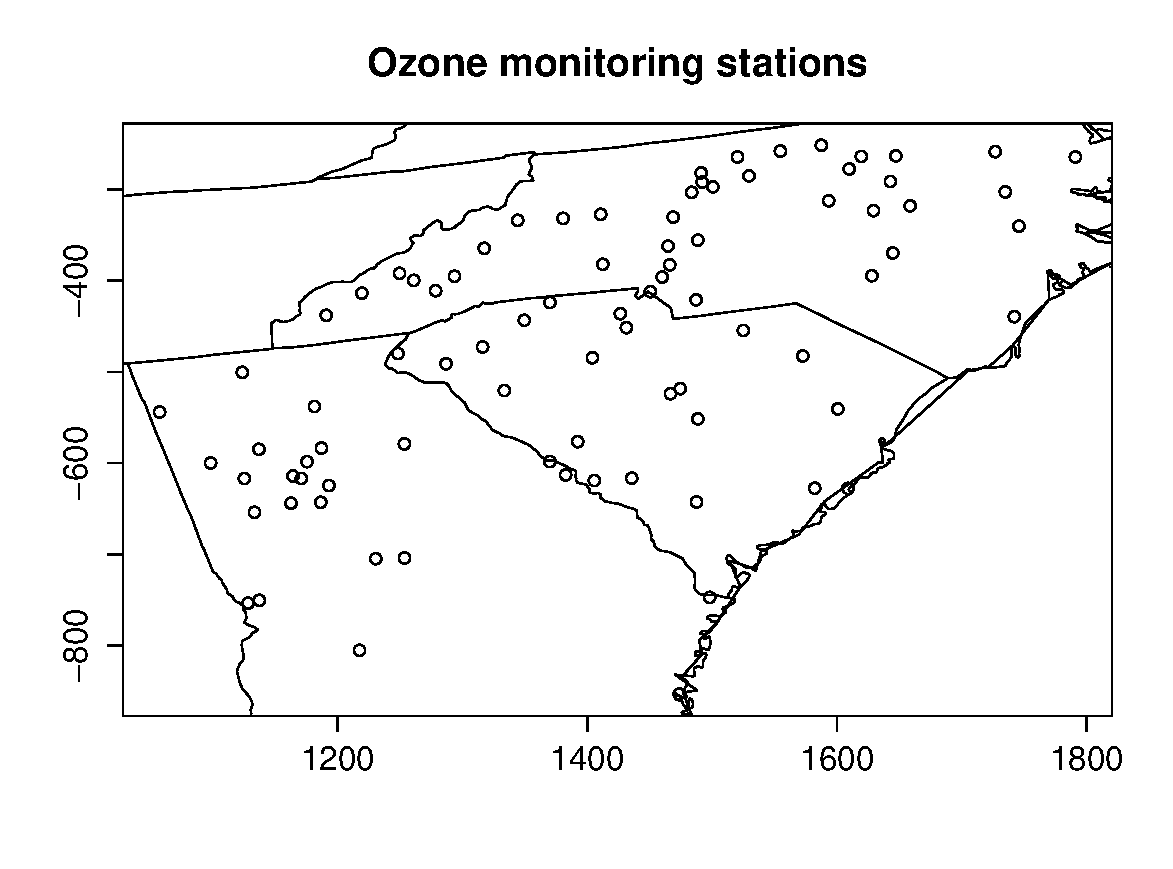
\includegraphics[width=0.8\linewidth]{./plots/ozone_station.pdf}

\end{frame}

\begin{frame}{Data analysis}
  \centering
  Max 8-hour ozone measurements at 85 sites in NC, SC, and GA for days 5 and 34.
    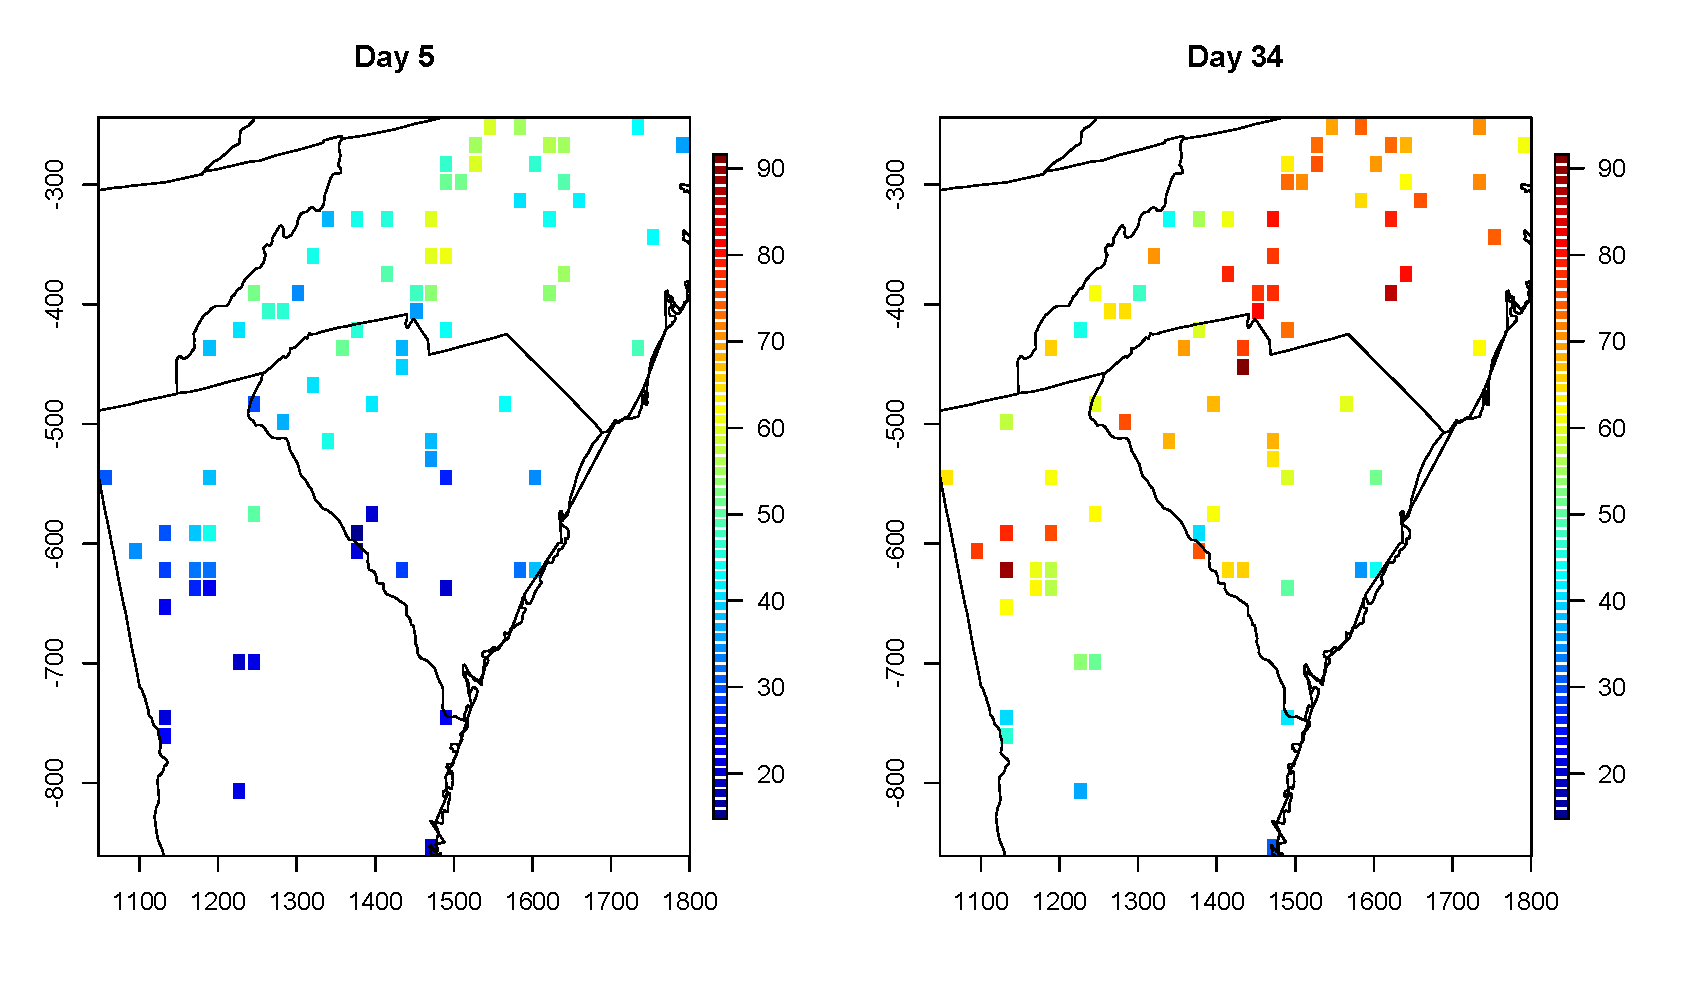
\includegraphics[width=1\linewidth]{./plots/ozone-day.pdf}

\end{frame}

\begin{frame}{Exploratory data analysis}
	\centering
	$\chi$-plot for residuals selected ozone sample quantiles
    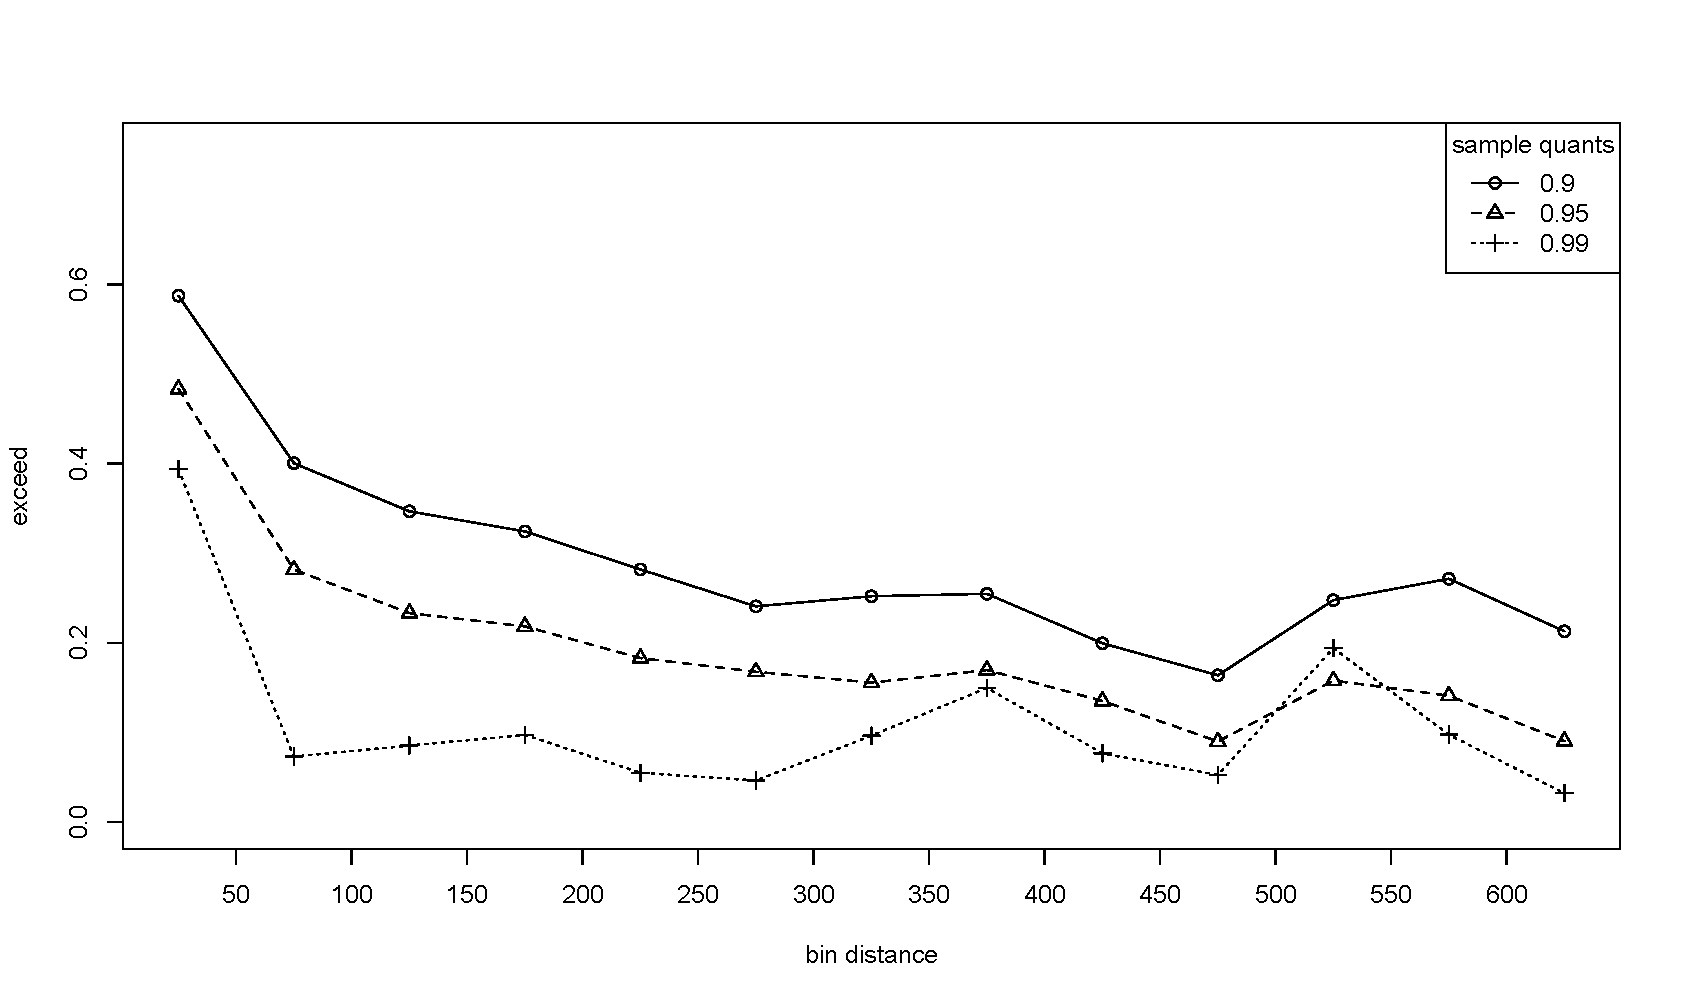
\includegraphics[width=1\linewidth]{./plots/chi-plot-ozone-res.pdf}
\end{frame}

\begin{frame}{Model comparisons}
  \begin{itemize} \setlength{\itemsep}{0.5em}
    \item 9 different analysis methods incorporating
    \begin{itemize}
      \item Gaussian vs $t$ vs skew-$t$ marginal distribution
      \item $K=1$ partition vs $K=5$ partitions
      \item No thresholding vs thresholding at $T=0.90$ sample quantile
    \end{itemize}
    \item All methods use a \Matern or exponential covariance ($\nu = 0.5$)
    \item Compare quantile and Brier scores using 5-fold cross validation (Gneiting and Raftery, 2007)
    \item Mean function modeled using a first-order spatial trend
  \end{itemize}
\end{frame}

\begin{frame}{Quantile score for cross-validation}
  \begin{itemize} \setlength{\itemsep}{0.5em}
    \item The quantile score for the $\tau$th quantile is
    \begin{align*}
      2 \{ I[y < \widehat{q}(\tau)] - \tau\} (\widehat{q} - y)
    \end{align*}
    where:
    \begin{itemize}
      \item $y$ is a test set value
      \item $\widehat{q}(\tau)$ is the estimated $\tau$th quantile
    \end{itemize}
  \end{itemize}
\end{frame}

\begin{frame}{Brier score}
  \begin{itemize} \setlength{\itemsep}{0.5em}
	\item The Brier score for predicting exceedance of threshold $c$ is
	\begin{align*}
	  [e(c) - P(c)]^2
	\end{align*}
	where 
	\begin{itemize}
		\item $y$ is a test set value
		\item $e(c) = I[y > c]$
		\item $P(c)$ is the predicted probability of exceeding $c$
	\end{itemize}
  \end{itemize}
\end{frame}

\begin{frame}{Five-fold cross-validation results}
  \begin{table}[htbp]
    \small
    \centering
    \begin{tabular}{l|c|r|rrrrr}
          \multicolumn{3}{c}{\ } & \multicolumn{5}{c}{Quantile}\\
           \hline
  Marginal & $K$ & $T$  & 0.900 & 0.950 & 0.990 & 0.995 & 0.999\\
  \hline
Gaussian & 1 & 0 & 16.38 & 15.76 & 14.52 & 14.08 & 13.22\\
$t$ & 1 & 0 & 16.15 & 15.51 & 14.00 & 13.43 & 12.32\\
$t$ & 5 & 0 & 13.61 & 12.66 & 10.96 & 10.40 & 9.34\\
skew $t$ & 1 & 0 & 9.24  & 7.27 & 4.13  & 3.27  & 1.96\\
skew $t$ & 5 & 0 & 15.81 & 14.46 & 11.57 & 10.57 & 8.60\\
$t$ & 1 & 0.9 & 5.52  & 3.58  & 1.77  & 1.47  & 1.10\\
$t$ & 5 & 0.9 & 5.98  & 4.27  & 2.41  & 2.03  & 1.49\\
 skew $t$ & 1 & 0.9 & {\bf 4.91}  & {\bf 3.16} & {\bf 1.45}  & {\bf 1.16}  & {\bf 0.82}\\
skew $t$ & 3 & 0.9 & 5.58 & 3.78 & 1.93& 1.58& 1.11\\
\hline
    \end{tabular}
  \end{table}
  \begin{itemize}
  	\item Brier score results are similar.
  \end{itemize}
\end{frame}

\begin{frame}{Simulation study}
  \begin{itemize} \setlength{\itemsep}{0.5em}
    \item 6 different data settings:
    \begin{itemize}
    	\item Gaussian vs $t$ vs skew-$t$ marginal distribution
        \item $K=1$ partition vs $K=5$ partitions
    \end{itemize}
    \item Results are similar to the results from the data analysis
    \item Biggest gains come from thresholding.
    \item Using skew models give additional gain, but small relative to gain for thresholding.
  \end{itemize}
\end{frame}

\begin{frame}{Future work}
  \begin{itemize} \setlength{\itemsep}{0.5em}
    \item Comparison with extreme value analysis methods
    \item Reporting of compliance with EPA ozone standards
    \item Including time in the model via standard spatiotemporal Gaussian models.  
  \end{itemize}
\end{frame}

\begin{frame}{Questions}
  \begin{itemize} \setlength{\itemsep}{0.5em}
    \item Questions?
    \item Thank you for your attention.
    \item Acknowledgment: This work was funded by EPA STAR award R835228.
  \end{itemize}
\end{frame}

\begin{frame}{References}
  \begin{itemize} \setlength{\itemsep}{0.5em}
    \item Demarta, S. and McNeil, A. J. (2007) The $t$ copula and related copulas. {\it International Statistical Review}, {\bf 73}, 111--129.
    \item Huser, R. and Davison, A. C. (2014) Space-time modelling of extreme events. {\it Journal of the Royal Statistical Society: Series B (Statistical Methodology)}, {\bf 76}, 439--461.
    \item Padoan, S. A. (2011) Multivariate extreme models based on underlying skew-$t$ and skew-normal distributions. {\it Journal of Multivariate Analysis}, {\bf 102}, 977--991.
    \item Zhang, H. and El-Shaarawi, A. (2010) On spatial skew-Gaussian processes and applications. {\it Environmetrics}, {\bf 21}, 33--47.
  \end{itemize}
\end{frame}

\end{document}